\documentclass{article}
\usepackage{graphicx}
\usepackage[margin=1.5cm]{geometry}
\usepackage{amsmath}

\begin{document}
\twocolumn

\title{History of Science in Latin America (INTD262): Essay Structure}
\author{Prof. Jordan C. Hanson}

\maketitle

\section{The Purpose of this Essay}

Writing this essay serves two goals.  First, we want to learn about the scientific discoveries, expeditions, and researchers of Latin America in the period between 1500-1900.  Second, we want to understand the science itself.  Thus, it is not sufficient to merely state what scientific results were obtained by Latin Americans in this period, but to share why these scientific claims must be true.  To meet this second goal, we must accomplish three tasks within the scientific topic.  First, we must apply the scientific attitude to our topic.  Second, we must demonstrate a quantitative understanding of the scientific principles at work within the discovery, expedition, or work of a researcher.  Third, we must provide the evidence the work produced.  This is a tall order for a 5000 word essay.

\section{The Prompt for the Assignment}

According to our syllabus, the prompt of this essay is

\begin{quote}
Select a major Latin American scientific discovery, expedition, or researcher. Using the course texts and bibliographies within them, expand upon the scientific history of the discovery, expedition, or researcher. Include the historical context of the work, the methodology, and the important results of the work.
\end{quote}

The prompt is a starting point.  The prompt is not meant to be restrictive.  However, an essay will be marked down significantly if it is missing specific requirements made in the prompt.  Here, there are essentially two requirements.  First, the essay must address the scientific results and historical context.  Second, the essay must address the methodology of the science.

\section{The Research before the Writing}

To produce a quality essay, it is imperative that we do our research and reading before doing any writing or planning.  At the end of each chapter in our course reading, we find bibliographies that point to sources of information about our topics.  Wardman Libary has a wealth of literature on our course topic, as does the Chicano Resource Center in the East LA Library.  While sources like Wikipedia are not prohibited, we should dive more deeply into our topics than a cursory internet search.

Here is list of books we have on loan from the Chicano Resource Center in SLC 212:

\begin{itemize}
\item \textit{Skywatchers of Ancient Mexico} - Anthony Aveni
\item \textit{Aztec Thought and Culture} - Miguel Le\'{o}n-Portilla
\item \textit{Archaeoastronomy in Pre-Columbian American} - Edited by Anthony Aveni
\item \textit{The Learned Ones: Nahua Intellectuals in Postconquest Mexico} - Kelly McDonough
\item \textit{Native American Astronomy} - Edited by Anthony Aveni
\end{itemize}

\section{The Importance of Creating an Outline}

It is imperative to structure our ideas for this essay.  Careful planning is required to satisfy the twin goals of the essay.  One useful tool for mapping the way a set of ideas are related is \verb+coggle.it+.  This is a web-based application that allows us to create visual outlines.  One example from a different course is shown in Fig. \ref{fig:1}.  Using a mapping tool like \verb+coggle.it+ will make outline creation more efficient.

\begin{figure}[hb]
\centering
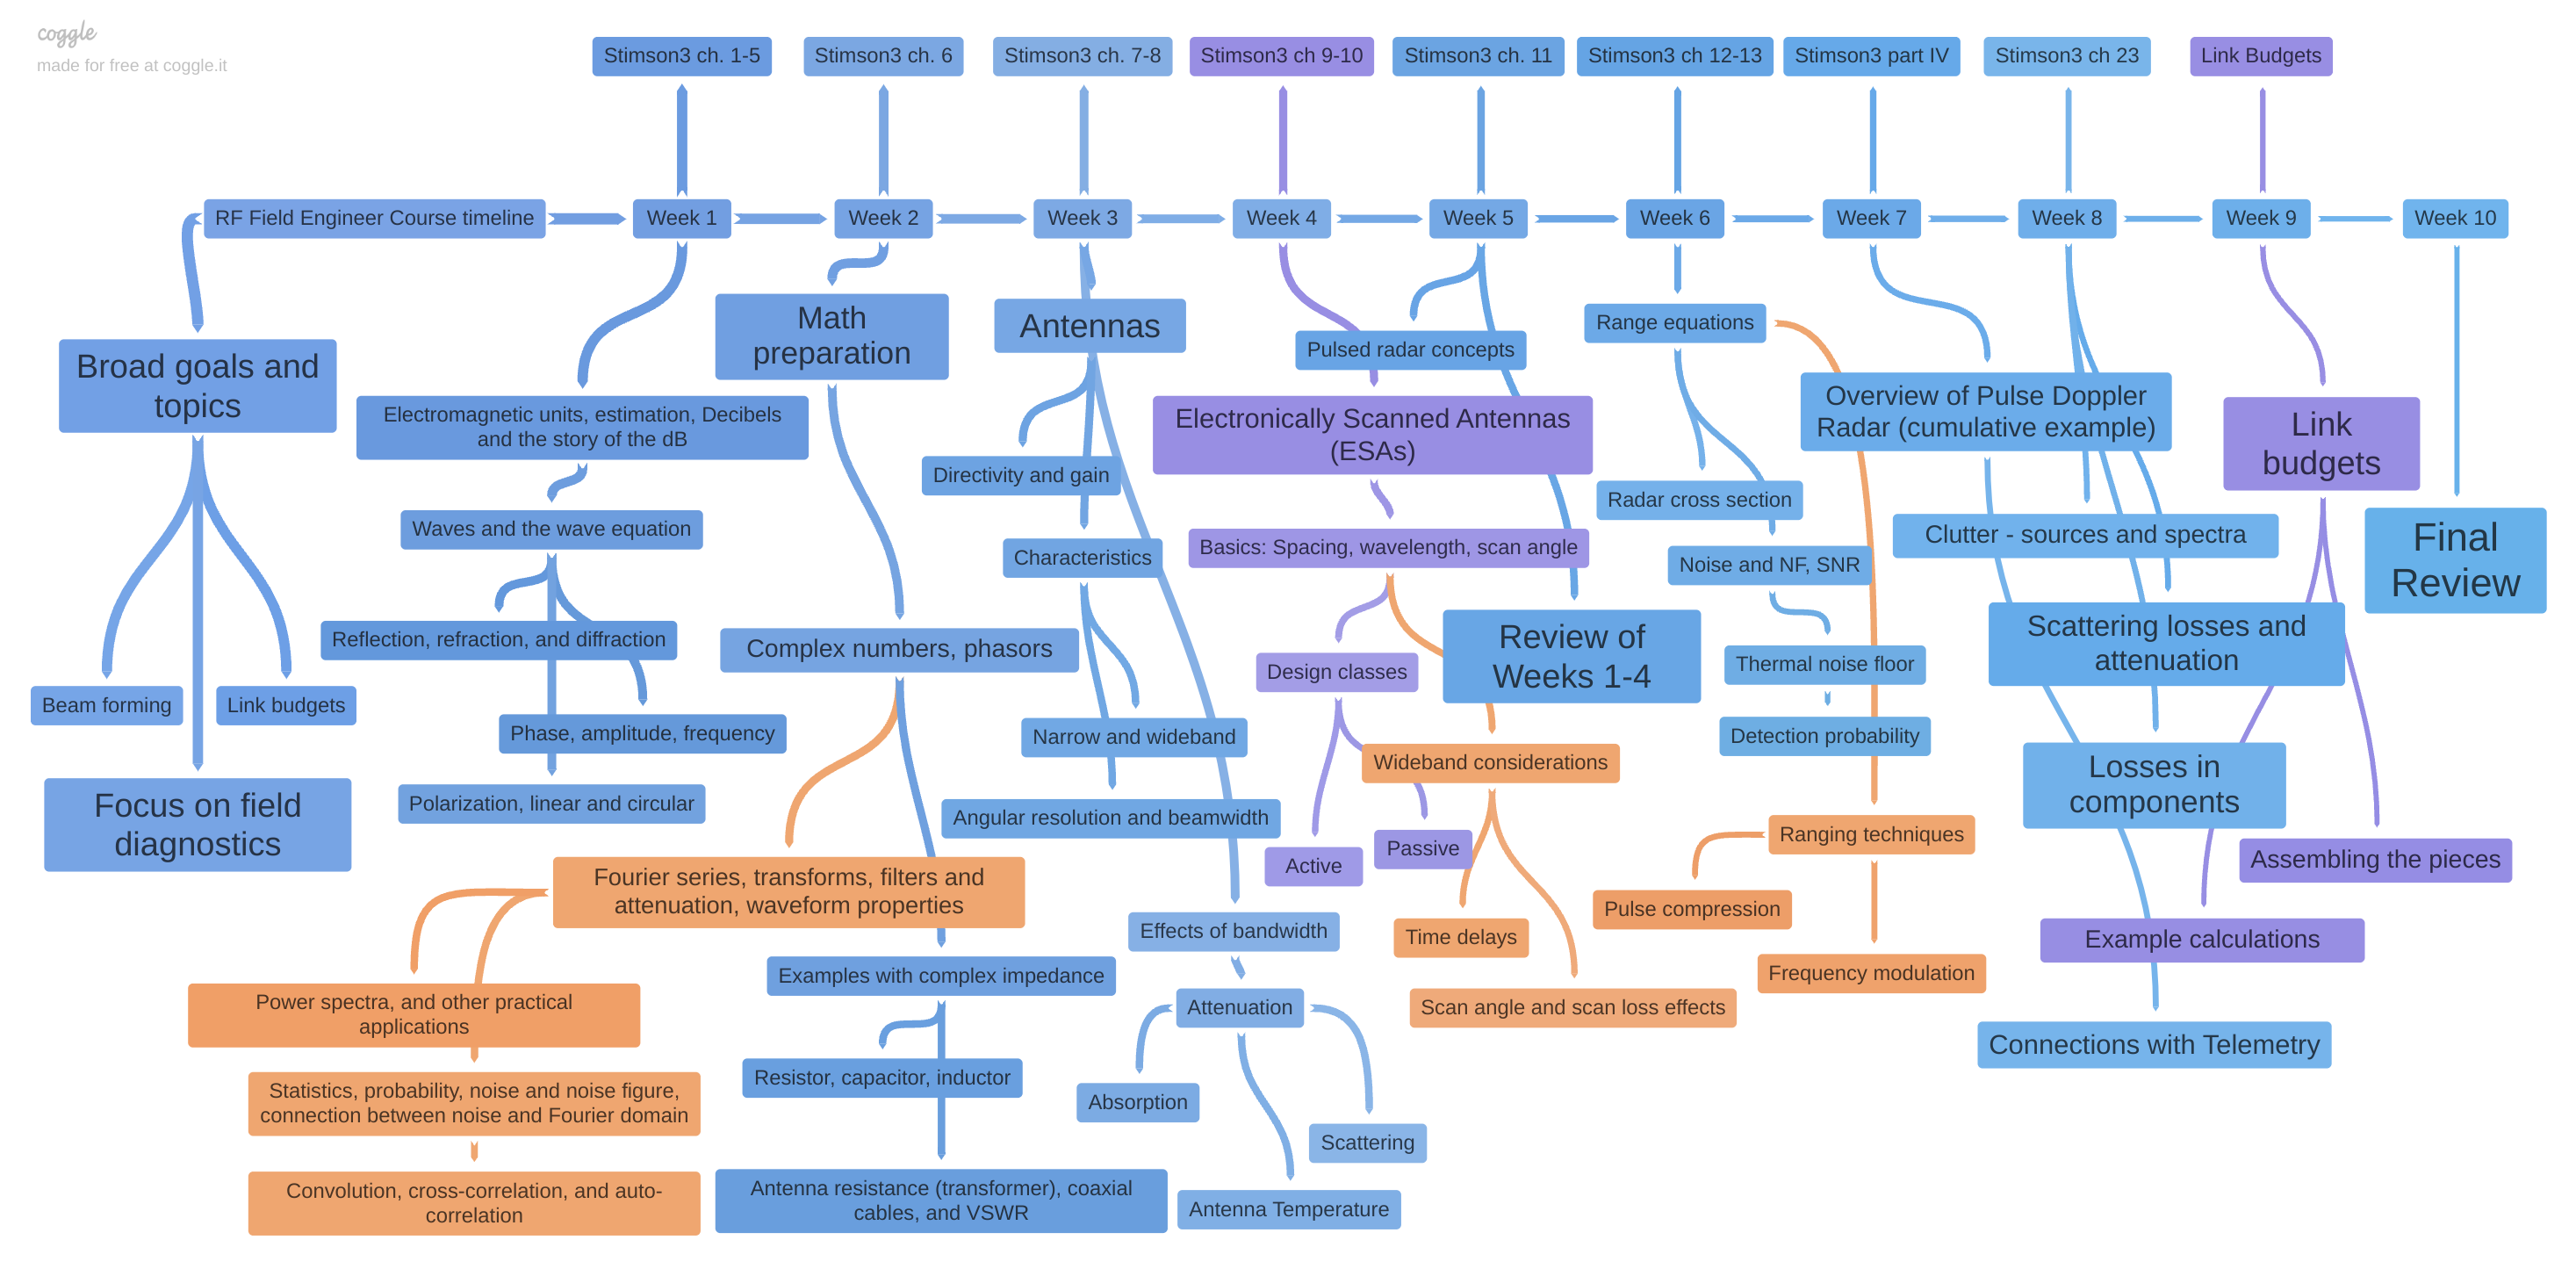
\includegraphics[width=0.5\textwidth]{RF_Field_Engineer_Course_timeline.png}
\caption{\label{fig:1} A map of the ideas for an engineering course.  The rectangles along the top are weeks, including midterm review and final review weeks.  Subtopics branch from the weeks.}
\end{figure}

For an essay that has several requirements, it is important to structure the work.  Before writing significant tracts of the essay, make decisions about how the ideas will fit together, and how the overall logical thread of the essay will progress.  With the structure and logical order of ideas in place, writing tracts of the essay will be easier and more clear.

\end{document}

Essay on Discovery, Expedition, or Researcher
- due November 1st, 2025
(a) Format: essays will be approximately 5,000 words,
and can be enhanced with figures, diagrams, maps,
and charts.
(b) Protocol: submit via PDF on Moodle
(c) Editing/drafts: please use the booking link (above
in contact info) to schedule office hours appoint-
ments. Students can use these appointments to
improve the content and structure of the paper.
(d) Prompt: “Select a major Latin American scien-
tific discovery, expedition, or researcher. Using
the course texts and bibliographies within them,
expand upon the scientific history of the discov-
ery, expedition, or researcher. Include the histor-
ical context of the work, the methodology, and
the important results of the work.”
